\newpage


\section{Information retrieval}
\label{sec:ir}

% \subsection{Problem statement}

Information Retrieval (IR) across an unstructured network is a graph search problem\cite{lv2002search}. Distributed search algorithms are designed to successfully locate resources while incurring low overhead (in time, space and message complexity)\cite{bisnik2005walk}.

In structured networks, the network topology can be exploited to increase search efficiency, this is not possible in an unstructured topology\cite{khatibi2021rd, li2005searching}. Hence, efficiently retrieving information is non-trivial in an unstructured network.

%A common `naive' approach in unstructured peer-to-peer information retrieval is to use Breadth-first search (BFS). While this has the benefit of simplicity, it floods the network with queries\cite{thampi2010replication}. Methods can be used to improve the performance of `naive' BFS such as including a time-to-live (ttl) for each query and implementing heuristics and metadata (see intelligent/directed BFS)\cite{tsoumakos2003p2pIr}. There are also significantly more efficient probabilistic approaches, e.g.\ random BFS, but those do not guarantee a full search through the network.

In short, the question can be posed as: how to find information quickly and efficiently while relying on a partial view of the network (the limited information available to a node) and not on a central repository of global knowledge. Solutions to this problem can be divided into two primary categories\cite{thampi2010replication}: blind, and informed.

% Not sure about this but could be good
% Inspired by Lamport's statement ``the popularity of the dining philosophers problem taught me that the best way to attract attention to a problem is to present it in terms of a story" we shall use the analogy of finding a book in a library to discuss information retrieval. Libraries are efficient for finding and retrieving a book as they are typically organised by a person, a librarian, with a global view of the system - without a consistent approach to organisation a library cannot be structured and the efficient mechanisms to search for a book within the library fail.
% even enforcing an alphabetical scheme to help make retrieval faster would require centralisation as we would need a node to allocate letters of the alphabet to each node entering the network

%One should make the distinction between locating and retrieving a known resource (i.e., searching by unique identifier) and searching for an unknown resource that may contain the desired information (i.e., a search engine). These are two distinct problems, in this case we are devising a solution for retrieving a specified piece of information and not designing a decentralised search engine.

% The IR module is intrinsically ties to the Persistent storage module as for IR to be necessary, the network needs to store information and the protocol for storing information dictates how information is identified. 

% Keys to improving the speed and efficiency of the information retrieval mechanism is to minimize the communication costs, that is, the number of messages sent between the peers, and to minimize the number of peers that are queried for each search request. 

\subsection{Related work}

In this section we present several techniques for information retrieval of a specified document on an unstructured peer-to-peer network. Typically flooding, random walks or expanding-rings are used to retrieve information stored by peers. Each peer visited will evaluate the query locally on its own content, and will support complex queries\cite{lua2005survey}.

\subsubsection{Gnutella `naive' breadth-first search}

BFS is the technique that was originally used in the Gnutella network and is illustrated in Figure~\ref{fig:gnutella}. The BFS search protocol in a peer-to-peer network is as follows: a querying node generates a $QUERY$ message which is propagated to all its known hosts. When a peer receives a $QUERY$ request, it searches its local storage for a match. If no match is found, it forwards the $QUERY$ to all of its known hosts (other than the sender). If some node $q$ receives the $QUERY$ and has a match in its local storage, $q$ generates a $QUERYHIT$ message to transmit the document. $QUERYHIT$ messages are sent along the same path that carried the $QUERY$ message\cite{zeinalipour2004ir}.

%When node $q$ receives a $QUERYHIT$ from more than one peer, it may decide to download the file from the peer with the best network connectivity.

\subsubsection{Extension to BFS with time-to-live}

The original Gnutella implementation of BFS sacrifices performance and network utilisation for the sake of simplicity. Each query consumes excessive network and processing resources because a query is propagated along all links (including nodes with high-latency)\cite{zeinalipour2004information}. This means a low bandwidth node can easily become a bottleneck. This became apparent as the Gnutella network became more popular and the search mechanisms failed to scale. One technique to avoid overusing network bandwidth is to associate each query with a time-to-live (TTL) parameter. The TTL parameter determines the maximum number of hops that a given query should be forwarded. In a typical value for the TTL is usually 7 and is decremented each time the query is forwarded. When the TTL becomes 0, the message is dropped. Note, some existing documents may not be located due to limited TTL\@.

\subsubsection{Random Breadth-first search technique}

Kalogeraki and Gunopulos propose an alternative to BFS, namely Random breadth-first search (RBFS) and evaluate its performance\cite{kalogeraki2002local}. They state that it can be a ``dramatic improvement over the `naive' BFS approach". In RBFS, a peer forwards a $QUERY$ to a random subset of its known hosts. The size of the subset can be a user specified parameter. The researchers suggest half of the peers ($0.5$) as in testing it proved the best compromise between IR success and message generation. RBFS, like the BFS mechanism, allows nodes to make local decisions quickly since they only needs to select a portion of their known hosts. However, this algorithm is probabilistic. It is possible that some large segments of the network may be unreachable because a node was unable to understand that a particular link would lead the query to a large segment of the network.\cite{zeinalipour2004information}

% \subsubsection{Random walker technique}

% The random walkers algorithm was originally proposed in 2002\cite{lv2002search}. The idea behind the approach is similar to that of RBFS. In Random walker, each node forwards a query message, called walker, randomly to one of its peers. To reduce the time to receive the results the idea of the walker is extended to a k-walker which after T steps is expected to reach approximately the same number of nodes as a 1-walker after kT steps. To prevent `walking' over the same nodes several times each node may retain states. The difference between RBFS and Rabdom walker is subtle, in RBFS each node forwards a query message to a fraction of its neighbors while in Random walker it is a specified conatnt of $k$. This results in the message complexity of RBFS remaining expentianl exponential, depsite being significantly more efficient than `naive' BFS, while in the k-Walker model the messages used is linear.

\subsubsection{Directed BFS with `Most Results in Past' heuristic}

In a directed BFS approach, each node forwards a query to a subset of its peers based on some heuristic. This technique was originally proposed by Yang et al. They compared a number of query routing heuristics and found that the `Most Results in Past' ($>RES$) heuristic was the most `satisfactory'\cite{yang2002efficient}. In other words, more documents were found in less steps using this heuristic. In $>RES$ a peer $q$ forwards a search message to $n$ peers which returned the most results for the last $k$ queries. In their experiments they chose $n=1$ and $k=10$ effectively turning Directed BFS into a directed Depth-first-search (DFS) approach. This technique may perform well because it routes queries to the larger network segments (which subsequently may also contain more relevant answers)\cite{zeinalipour2004information}.

\subsubsection{Intelligent Search Mechanism}

The Intelligent Search Mechanism (ISM) is a more sophisticated approach to Directed BFS with `Most Results in Past' heuristic\cite{kalogeraki2002local}. In an effort to minimise the number of queries made and improve search performance a peer estimates, for each query, which of its peers are more likely to reply to the query, and propagates the query message to those peers only. The mechanism consists of two components: a \textit{profiling mechanism} used by a node to build a profile of its known hosts (neighbouring peers) and a \textit{relevance rank} that uses the peer’s profiles to select the neighbours that will lead a query to the most relevant answers.
% The profiling mechanism is used to maintain the most recent queries, the corresponding queryhits along with the number of results.

\subsubsection{Gossiping to replicate global state}

A different approach to those previously discussed is, instead of searching based on a partial view of the network, to maintain a global state in a decentralised fashion using randomised gossipping. Cuenca-Acuna and Nguyen suggest an approach to constructing a content addressable publish/subscribe service that uses gossiping of global state across unstructured communities\cite{cuenca2002text}. Their framework is based on a global inverted index, i.e.\ a globally maintained map of content to its location. The inverted index is partially constructed by each node $n_k$, specifically, $n_k$ constructs a bloom filter $b_k$, of its local index and propagates it to the rest of the network using gossiping. A bloom filter is a space-efficient probabilistic data structure that is used to test whether an element is a member of a set, in this case it is an efficient way of representing if $n_k$ hosts the information. While this is an interesting approach, the paper does state that the technique does not scale and maintaining a global state across nodes may not be suitable for large network.\cite{zeinalipour2004ir}
% The global inverted index is then the collection of each node's bloom filters. Bloom filters are an attractive approach for distributed environments because they achieve smaller messages.

\subsection{Design \& implementation}

Gnutella showed us that a `naive' BFS is not a practical solution, as it floods the network with queries and so scales poorly for large networks. It is specially impractical as without a TTL there is no upper-bound to the breadth of search for a query. Each search query requires excessive network use and processing resources as a query is propagated along all links (including high latency links)\cite{zeinalipour2004ir}.

%Some particularly efficient solutions make use of structured elements such as super-peers, but, these approaches will not be considered as they re-introduce elements of centralisation.

%Blind search makes use of flooding techniques to relay queries to peers, where peers maintain no information about the P2P network or probable locations of objects(used in GNutella\cite{GNutella}). The informed search on the other hand maintains routing information based on popularity of objects, success rate, etc.  Despite better performance, due to the high overhead cost of informed search it is not being considered in this paper\cite{comparison_of_P2P_search}.

%It has been proven experimentally that random walk is better than randomised flooding for information retrieval\cite{walk_search}, in the condition of Peer clustering, where there are communities in the topology, with dense connectivity between Peers in the same group and sparse connectivity between Peers of different groups. ?need to say its relevant maybe? In the case of flooding, a user request is re-issued by the user(or the system on behalf of the user) multiple times in hopes of locating more resources, whereas the usage of `random walk' algorithm follows completely different trajectories and has a higher chance of locating new resources.

The design and implementation of the Butter Information retrieval (IR) module is largely inspired by the work carried out on later version of the Gnutella project (discussed in Chapter~\ref{ch:relatedProjects}). We did not implement a semi-centralised peer-to-peer architecture such as BitTorrent as by reintroducing centralised elements, in an effort to increase search efficiency, the resulting network is less fault-tolerant and hence less dependable. On the other hand, Butter's IR module needs to retrieve information efficiently in regard to time and message complexity to make application services built using the framework usable.

Butter implements a RBFS technique with a user specified TTL (per query). Having a user specified TTL allows the user to define how far they are willing to go to fetch a piece of information. Users also have the option to use a BFS mechanisms if the information is not found using the default RBFS mechanisms.

\begin{figure}[ht]
    \centering
    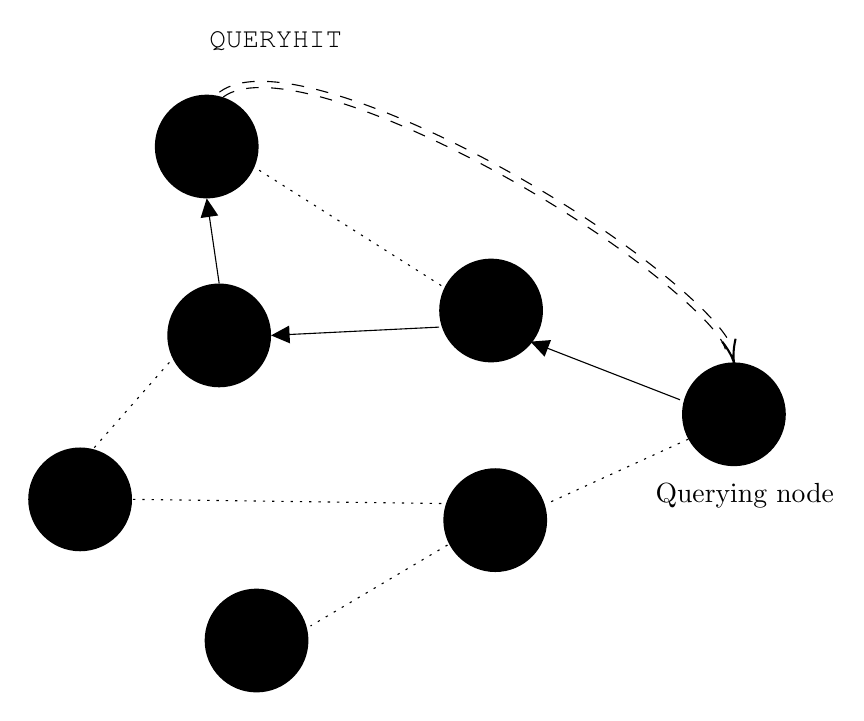
\begin{tikzpicture}[x=0.75pt,y=0.75pt,yscale=-1,xscale=1]
%uncomment if require: \path (0,451); %set diagram left start at 0, and has height of 451

%Shape: Circle [id:dp9331094894799612] 
    \draw  [draw opacity=0][fill={rgb, 255:red, 0; green, 0; blue, 0 }  ,fill opacity=1 ] (119,249) .. controls (119,235.19) and (130.19,224) .. (144,224) .. controls (157.81,224) and (169,235.19) .. (169,249) .. controls (169,262.81) and (157.81,274) .. (144,274) .. controls (130.19,274) and (119,262.81) .. (119,249) -- cycle ;
%Shape: Circle [id:dp9877389362602726]
    \draw  [draw opacity=0][fill={rgb, 255:red, 0; green, 0; blue, 0 }  ,fill opacity=1 ] (317,158) .. controls (317,144.19) and (328.19,133) .. (342,133) .. controls (355.81,133) and (367,144.19) .. (367,158) .. controls (367,171.81) and (355.81,183) .. (342,183) .. controls (328.19,183) and (317,171.81) .. (317,158) -- cycle ;
%Shape: Circle [id:dp0016664462798891]
    \draw  [draw opacity=0][fill={rgb, 255:red, 0; green, 0; blue, 0 }  ,fill opacity=1 ] (319,259) .. controls (319,245.19) and (330.19,234) .. (344,234) .. controls (357.81,234) and (369,245.19) .. (369,259) .. controls (369,272.81) and (357.81,284) .. (344,284) .. controls (330.19,284) and (319,272.81) .. (319,259) -- cycle ;
%Shape: Circle [id:dp3393753853906585]
    \draw  [draw opacity=0][fill={rgb, 255:red, 0; green, 0; blue, 0 }  ,fill opacity=1 ] (180,79) .. controls (180,65.19) and (191.19,54) .. (205,54) .. controls (218.81,54) and (230,65.19) .. (230,79) .. controls (230,92.81) and (218.81,104) .. (205,104) .. controls (191.19,104) and (180,92.81) .. (180,79) -- cycle ;
%Shape: Circle [id:dp6653810548572199]
    \draw  [draw opacity=0][fill={rgb, 255:red, 0; green, 0; blue, 0 }  ,fill opacity=1 ] (434,208) .. controls (434,194.19) and (445.19,183) .. (459,183) .. controls (472.81,183) and (484,194.19) .. (484,208) .. controls (484,221.81) and (472.81,233) .. (459,233) .. controls (445.19,233) and (434,221.81) .. (434,208) -- cycle ;
%Straight Lines [id:da22721998614149208]
    \draw    (433,201) -- (363.8,174.09) ;
    \draw [shift={(361,173)}, rotate = 21.25] [fill={rgb, 255:red, 0; green, 0; blue, 0 }  ][line width=0.08]  [draw opacity=0] (8.93,-4.29) -- (0,0) -- (8.93,4.29) -- cycle    ;
%Shape: Circle [id:dp23503433874211244]
    \draw  [draw opacity=0][fill={rgb, 255:red, 0; green, 0; blue, 0 }  ,fill opacity=1 ] (186,170) .. controls (186,156.19) and (197.19,145) .. (211,145) .. controls (224.81,145) and (236,156.19) .. (236,170) .. controls (236,183.81) and (224.81,195) .. (211,195) .. controls (197.19,195) and (186,183.81) .. (186,170) -- cycle ;
%Curve Lines [id:da8258695712571896]
    \draw  [dash pattern={on 4.5pt off 4.5pt}]  (211.1,52.8) .. controls (215.83,49.25) and (222.64,47.57) .. (231.07,47.57) .. controls (255.64,47.57) and (294.25,61.83) .. (332.86,81.67) .. controls (356.91,94.02) and (380.97,108.53) .. (401.61,123.04) .. controls (432.52,144.78) and (455.66,166.59) .. (457.83,175.9)(212.9,55.2) .. controls (217.2,51.97) and (223.44,50.57) .. (231.07,50.57) .. controls (255.32,50.57) and (293.4,64.77) .. (331.49,84.33) .. controls (355.42,96.63) and (379.35,111.06) .. (399.88,125.5) .. controls (430.01,146.68) and (452.89,167.79) .. (454.87,176.66) ;
    \draw [shift={(459,183)}, rotate = 257.2] [color={rgb, 255:red, 0; green, 0; blue, 0 }  ][line width=0.75]    (10.93,-3.29) .. controls (6.95,-1.4) and (3.31,-0.3) .. (0,0) .. controls (3.31,0.3) and (6.95,1.4) .. (10.93,3.29)   ;
%Straight Lines [id:da49607654384730693]
    \draw  [dash pattern={on 0.84pt off 2.51pt}]  (318,146) -- (228,89) ;
%Straight Lines [id:da7736178088954417]
    \draw    (317,166) -- (239,169.85) ;
    \draw [shift={(236,170)}, rotate = 357.17] [fill={rgb, 255:red, 0; green, 0; blue, 0 }  ][line width=0.08]  [draw opacity=0] (8.93,-4.29) -- (0,0) -- (8.93,4.29) -- cycle    ;
%Straight Lines [id:da4613250022232429]
    \draw  [dash pattern={on 0.84pt off 2.51pt}]  (187,183) -- (150,225) ;
%Straight Lines [id:da5738181000901116]
    \draw  [dash pattern={on 0.84pt off 2.51pt}]  (437,220) -- (369,251) ;
%Shape: Circle [id:dp11048151315696086]
    \draw  [draw opacity=0][fill={rgb, 255:red, 0; green, 0; blue, 0 }  ,fill opacity=1 ] (204,317) .. controls (204,303.19) and (215.19,292) .. (229,292) .. controls (242.81,292) and (254,303.19) .. (254,317) .. controls (254,330.81) and (242.81,342) .. (229,342) .. controls (215.19,342) and (204,330.81) .. (204,317) -- cycle ;
%Straight Lines [id:da9165977584013065]
    \draw    (211,145) -- (205.43,106.97) ;
    \draw [shift={(205,104)}, rotate = 81.67] [fill={rgb, 255:red, 0; green, 0; blue, 0 }  ][line width=0.08]  [draw opacity=0] (8.93,-4.29) -- (0,0) -- (8.93,4.29) -- cycle    ;
%Straight Lines [id:da5283181536620382]
    \draw  [dash pattern={on 0.84pt off 2.51pt}]  (318,251) -- (169,249) ;
%Straight Lines [id:da7410818285653099]
    \draw  [dash pattern={on 0.84pt off 2.51pt}]  (321,271) -- (255,310) ;

% Text Node
    \draw (205,22) node [anchor=north west][inner sep=0.75pt]   [align=left] {{\fontfamily{pcr}\selectfont QUERYHIT}};
% Text Node
    \draw (420,240) node [anchor=north west][inner sep=0.75pt]   [align=left] {Querying node};


\end{tikzpicture}

    \caption{Successful RBFS on Butter}
    \label{fig:succesfulRBFS}
\end{figure}

\noindent The RBFS implementation in Butter is as follows:
\begin{itemize}
    \item A peer $i$ generates a $QUERY$ message which is propagated to a random subset of its neighbors (known hosts)
    \item When a peer $j$ receives a $QUERY$ request, it first checks if it possesses the queried data in its local repository.
    \begin{itemize}
        \item If it does, it returns the information with a $QUERYHIT$ message.
        \item Else, it propagates the $QUERY$ to a random subset of its neighbours
    \end{itemize}
\end{itemize}

The proportion of the known hosts selected can be user specified. If unspecified it defaults to $0.5$. An example successful run is illustrated in Figure~\ref{fig:succesfulRBFS}.

Butter stores information in a `chunk' data structure. which contains a 4kb array for information, some optional keywords to associate with that information, and a $part/totalParts$ number. If the data is smaller that 4kb then it is stored in a single chunk, else, when data is added to the network, it is broken down into several `chunks' with the appropriate part number.

Information is uniquely identified by the hash of the whole information and a chunk number. Initially a query search is based on the hashed information regardless of the chunk number, simply finding the first hash match. Once an initial hit is made, the querying node learns about the number of chunks and hence generates queries for all the remaining parts. This enables the rest of the search to be carried out in parallel and improves retrieval speed.

\subsection{Testing \& Evaluation}

Using the tested, we spawned nodes and stored random information strings in each of the nodes. We stored the information identifiers in a global database and then spawned another node to systematically query each of the spawned nodes. We measured the average number of messages generated, documents found as well as the average time taken for the `naive' BFS and RBFS with TTL search mechanisms.

\begin{table}[ht]
    \centering
    \begin{tabular}{|l|l|l|l|}
        \hline
        Technique & Avg number of messages & (\%) Documents found  & Avg time taken (seconds) \\
        \hline
        BFS       & 587               & 100                   & 10.1 \\
        RBFS      & 235                & 68                    & 5.4 \\
        \hline
    \end{tabular}
    \caption{Comparing information retrieval techniques. Carried out for 10 queries on 100 simulated nodes.}
    \label{tab:irTechniques}
\end{table}

\begin{figure}[ht]
    \centering
    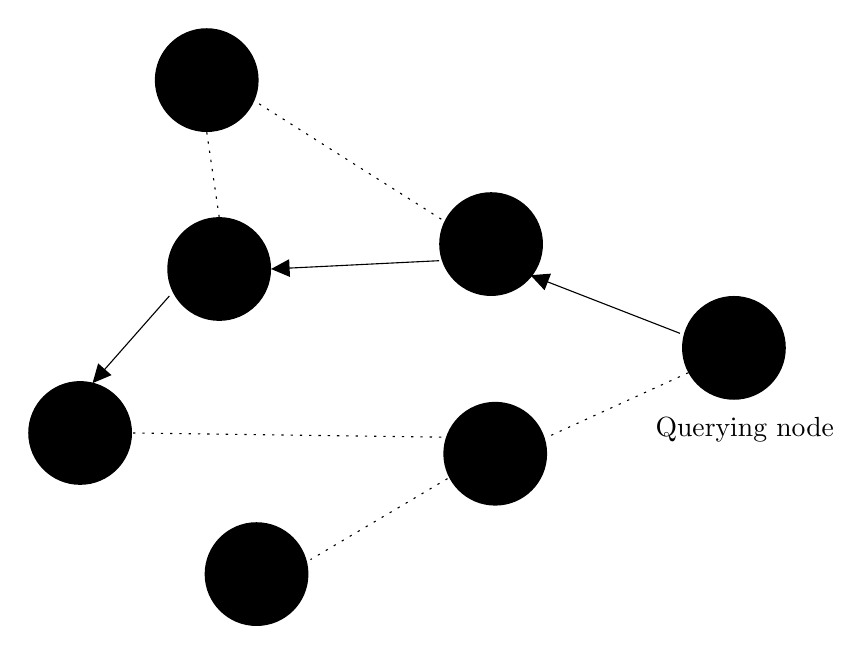
\begin{tikzpicture}[x=0.75pt,y=0.75pt,yscale=-1,xscale=1]
%uncomment if require: \path (0,451); %set diagram left start at 0, and has height of 451

%Shape: Circle [id:dp9331094894799612] 
    \draw  [draw opacity=0][fill={rgb, 255:red, 0; green, 0; blue, 0 }  ,fill opacity=1 ] (119,249) .. controls (119,235.19) and (130.19,224) .. (144,224) .. controls (157.81,224) and (169,235.19) .. (169,249) .. controls (169,262.81) and (157.81,274) .. (144,274) .. controls (130.19,274) and (119,262.81) .. (119,249) -- cycle ;
%Shape: Circle [id:dp9877389362602726] 
    \draw  [draw opacity=0][fill={rgb, 255:red, 0; green, 0; blue, 0 }  ,fill opacity=1 ] (317,158) .. controls (317,144.19) and (328.19,133) .. (342,133) .. controls (355.81,133) and (367,144.19) .. (367,158) .. controls (367,171.81) and (355.81,183) .. (342,183) .. controls (328.19,183) and (317,171.81) .. (317,158) -- cycle ;
%Shape: Circle [id:dp0016664462798891] 
    \draw  [draw opacity=0][fill={rgb, 255:red, 0; green, 0; blue, 0 }  ,fill opacity=1 ] (319,259) .. controls (319,245.19) and (330.19,234) .. (344,234) .. controls (357.81,234) and (369,245.19) .. (369,259) .. controls (369,272.81) and (357.81,284) .. (344,284) .. controls (330.19,284) and (319,272.81) .. (319,259) -- cycle ;
%Shape: Circle [id:dp3393753853906585] 
    \draw  [draw opacity=0][fill={rgb, 255:red, 0; green, 0; blue, 0 }  ,fill opacity=1 ] (180,79) .. controls (180,65.19) and (191.19,54) .. (205,54) .. controls (218.81,54) and (230,65.19) .. (230,79) .. controls (230,92.81) and (218.81,104) .. (205,104) .. controls (191.19,104) and (180,92.81) .. (180,79) -- cycle ;
%Shape: Circle [id:dp6653810548572199] 
    \draw  [draw opacity=0][fill={rgb, 255:red, 0; green, 0; blue, 0 }  ,fill opacity=1 ] (434,208) .. controls (434,194.19) and (445.19,183) .. (459,183) .. controls (472.81,183) and (484,194.19) .. (484,208) .. controls (484,221.81) and (472.81,233) .. (459,233) .. controls (445.19,233) and (434,221.81) .. (434,208) -- cycle ;
%Straight Lines [id:da22721998614149208] 
    \draw    (433,201) -- (363.8,174.09) ;
    \draw [shift={(361,173)}, rotate = 21.25] [fill={rgb, 255:red, 0; green, 0; blue, 0 }  ][line width=0.08]  [draw opacity=0] (8.93,-4.29) -- (0,0) -- (8.93,4.29) -- cycle    ;
%Shape: Circle [id:dp23503433874211244] 
    \draw  [draw opacity=0][fill={rgb, 255:red, 0; green, 0; blue, 0 }  ,fill opacity=1 ] (186,170) .. controls (186,156.19) and (197.19,145) .. (211,145) .. controls (224.81,145) and (236,156.19) .. (236,170) .. controls (236,183.81) and (224.81,195) .. (211,195) .. controls (197.19,195) and (186,183.81) .. (186,170) -- cycle ;
%Straight Lines [id:da49607654384730693] 
    \draw  [dash pattern={on 0.84pt off 2.51pt}]  (318,146) -- (228,89) ;
%Straight Lines [id:da7736178088954417] 
    \draw    (317,166) -- (239,169.85) ;
    \draw [shift={(236,170)}, rotate = 357.17] [fill={rgb, 255:red, 0; green, 0; blue, 0 }  ][line width=0.08]  [draw opacity=0] (8.93,-4.29) -- (0,0) -- (8.93,4.29) -- cycle    ;
%Straight Lines [id:da4613250022232429] 
    \draw    (187,183) -- (151.98,222.75) ;
    \draw [shift={(150,225)}, rotate = 311.38] [fill={rgb, 255:red, 0; green, 0; blue, 0 }  ][line width=0.08]  [draw opacity=0] (8.93,-4.29) -- (0,0) -- (8.93,4.29) -- cycle    ;
%Straight Lines [id:da5738181000901116] 
    \draw  [dash pattern={on 0.84pt off 2.51pt}]  (437,220) -- (369,251) ;
%Shape: Circle [id:dp11048151315696086] 
    \draw  [draw opacity=0][fill={rgb, 255:red, 0; green, 0; blue, 0 }  ,fill opacity=1 ] (204,317) .. controls (204,303.19) and (215.19,292) .. (229,292) .. controls (242.81,292) and (254,303.19) .. (254,317) .. controls (254,330.81) and (242.81,342) .. (229,342) .. controls (215.19,342) and (204,330.81) .. (204,317) -- cycle ;
%Straight Lines [id:da9165977584013065] 
    \draw  [dash pattern={on 0.84pt off 2.51pt}]  (211,145) -- (205,104) ;
%Straight Lines [id:da5283181536620382] 
    \draw  [dash pattern={on 0.84pt off 2.51pt}]  (318,251) -- (169,249) ;
%Straight Lines [id:da7410818285653099] 
    \draw  [dash pattern={on 0.84pt off 2.51pt}]  (321,271) -- (255,310) ;

% Text Node
    \draw (420,240) node [anchor=north west][inner sep=0.75pt]   [align=left] {Querying node};


\end{tikzpicture}

    \caption{Failed RBFS on Butter}
    \label{fig:failedRBFS}
\end{figure}

Table~\ref{tab:irTechniques} shows a clear improvement in message complexity using a RBFS approach over BFS. However, the \% of successfully retrieved documents is significantly lower. There is a compromise to be made between speed, message complexity and success rate. A failed scenario of RBFS is depicted in Figure~\ref{fig:failedRBFS}. The value of the proportion of known hosts selected at random could be tweaked from the default $0.5$ to other values to improve the success rate.

Two features mentioned in the Persistent storage section could have an impact on IR performance. We mention a node geotag enabling information to be spread geographically which in turn would improve resilience. This may also help minimise latency and hence improves search time. In addition, dynamic group sizes based on the perceived popularity of a piece information, i.e.\ information that is frequently queried, may increase the probability of a hit and spreads the load across more nodes, however, this would have to be further tested.

In their work Zeinalipour and Gunopulos\cite{zeinalipour2004information} have shown, we can greatly improve the \% successful document retrieval while maintaining similarly efficient message complexity to RBFS by using an informed approach. RBFS does not use any explicit technique to guide the search query to the most relevant content, which is a desirable property in information retrieval. A future implementation will look at implementing an informed approach; most probably the Intelligent Search Mechanism.

